\documentclass{article}
\usepackage{arxiv}

\usepackage[utf8]{inputenc}
\usepackage[T1]{fontenc}
\usepackage{hyperref}
\usepackage{url}
\usepackage{booktabs}
\usepackage{amsmath}
\usepackage{amssymb}
\usepackage{microtype}
\usepackage{graphicx}
\usepackage{xcolor}
\usepackage{listings}
\usepackage[numbers]{natbib}
\usepackage{CJKutf8}
\usepackage{tikz}
\usetikzlibrary{positioning, arrows.meta, fit, backgrounds}

% Accent palette (matches the ByteDance arXiv house style).
\definecolor{accent}{HTML}{2A5AA8}
\definecolor{pyaccent}{HTML}{B5651D}
\definecolor{pybg}{HTML}{FBF0E6}

\hypersetup{
  colorlinks=true,
  linkcolor=accent,
  citecolor=accent,
  urlcolor=accent,
  pdftitle={A Native Rust Re-implementation of the SIA Self-Improving-Agent Framework: Architecture, Fidelity, and Extensions},
  pdfauthor={Micah Stubbs, Will Stark},
}

% Suppress the arxiv.sty "A Preprint" marker (under-title text and page header).
\renewcommand{\undertitle}{}
\renewcommand{\headeright}{}

\makeatletter
% Colored section headers (ByteDance arXiv style), preserving arxiv.sty spacing.
\renewcommand{\section}{\@startsection{section}{1}{\z@}%
  {-2.0ex \@plus -0.5ex \@minus -0.2ex}{1.5ex \@plus 0.3ex \@minus 0.2ex}%
  {\large\bfseries\raggedright\color{accent}}}
\renewcommand{\subsection}{\@startsection{subsection}{2}{\z@}%
  {-1.8ex \@plus -0.5ex \@minus -0.2ex}{0.8ex \@plus 0.2ex}%
  {\normalsize\bfseries\raggedright\color{accent}}}
\renewcommand{\subsubsection}{\@startsection{subsubsection}{3}{\z@}%
  {-1.5ex \@plus -0.5ex \@minus -0.2ex}{0.5ex \@plus 0.2ex}%
  {\normalsize\bfseries\raggedright\color{accent}}}
\renewcommand{\paragraph}{\@startsection{paragraph}{4}{\z@}%
  {1.5ex \@plus 0.5ex \@minus 0.2ex}{-1em}{\normalsize\bfseries\color{accent}}}

% Clean title block: accent title, no heavy black bars (ByteDance style).
\renewcommand{\@toptitlebar}{\vskip 0.10in}
\renewcommand{\@bottomtitlebar}{\vskip 0.12in}
\renewcommand{\@maketitle}{%
  \vbox{%
    \hsize\textwidth \linewidth\hsize
    \vskip 0.1in
    \@toptitlebar
    \centering
    {\LARGE\scshape\color{accent} \@title\par}
    \@bottomtitlebar
    \vskip 0.05in
    \def\And{\end{tabular}\hfil\linebreak[0]\hfil\begin{tabular}[t]{c}\bfseries\rule{\z@}{24\p@}\ignorespaces}%
    \def\AND{\end{tabular}\hfil\linebreak[4]\hfil\begin{tabular}[t]{c}\bfseries\rule{\z@}{24\p@}\ignorespaces}%
    \begin{tabular}[t]{c}\bfseries\rule{\z@}{24\p@}\@author\end{tabular}%
    \vskip 0.35in \@minus 0.1in \center{\@date}\vskip 0.18in
  }%
}

% Colored, enclosed abstract: accent rule + heading + accent rule.
\renewenvironment{abstract}{%
  \par\vskip 0.05in
  {\color{accent}\hrule height 1pt}\vskip 7pt
  \centerline{\large\bfseries\color{accent} Abstract}\vskip 6pt
  \begingroup\leftskip 2.2em \rightskip 2.2em
}{%
  \par\endgroup\vskip 6pt {\color{accent}\hrule height 1pt}\vskip 0.12in
}
\makeatother

% Inline + block code styling (no external branding)
\definecolor{codeframe}{HTML}{B0B0B0}
\lstset{
  basicstyle=\footnotesize\ttfamily,
  breaklines=true,
  breakatwhitespace=false,
  columns=fullflexible,
  keepspaces=true,
  frame=single,
  rulecolor=\color{codeframe},
  framesep=5pt,
  xleftmargin=6pt,
  showstringspaces=false,
}

\title{A Native Rust Re-implementation of the SIA\\ Self-Improving-Agent Framework:\\ Architecture, Fidelity, and Extensions}

\author{%
  Micah Stubbs\thanks{This is a
  system-and-design / experience report on the \texttt{sia\_rust} codebase, not a
  results paper: its empirical content is limited to (a) differential byte-parity
  tests against the reference Python implementation, (b) deterministic
  microbenchmarks, and (c) offline unit/integration tests. End-to-end
  self-improvement accuracy studies are explicitly future work. All quantitative
  claims are drawn from artifacts in the repository and cited to their source.}\\
  Superradiant\\
  \texttt{micah@superradiant.ai}
  \And
  Will Stark\\
  Superradiant\\
  \texttt{will@superradiant.ai}
}

\date{\today}

\begin{document}
\begin{CJK}{UTF8}{gbsn}
\maketitle

\begin{abstract}
SIA (Self-Improving AI with Harness \& Weight Updates) is a framework in which a
Meta-Agent writes and improves a Target-Agent, the Target-Agent executes a task,
and a Feedback-Agent analyzes the resulting trajectory to propose the next
improvement \citep{hebbar2026sia}. This paper is a system and experience report on
\texttt{sia\_rust}, a native Rust re-implementation of the SIA framework plus a set
of safety, observability, and scheduling extensions.

We describe three bodies of work. First, a \textbf{faithful port} of the
deterministic SIA core (orchestrator, context/trajectory management, prompt system,
run-directory format, and web visualizer) that reproduces the reference Python
implementation's prompt, context, and execution-log outputs \textbf{byte-for-byte},
verified by a differential-parity harness over an ASCII + CJK + emoji +
control-character matrix. Second, a \textbf{native multi-provider LLM agent-runner
layer} built on \texttt{rig-core} and injectable HTTP transports, comprising three
runners (a Claude \texttt{/v1/messages} tool-use loop, an OpenHands-style
OpenAI-compatible loop, and a PydanticAI-style loop), with trajectory-capture
middleware, a provider/profile mapping layer, retry/resilience decorators, and a
structured-output parity harness --- the entire LLM layer is feature-gated and
driven through injectable transports so its full tool-use loops are tested offline
with scripted responses. Third, a set of \textbf{extensions} scoped honestly as
engineering primitives and seams: a pure-\texttt{std} capability allow-list and a
formal threat model for self-modifying agents; a native \texttt{Verifier} trait
with adversarial-robustness hooks; per-generation telemetry; an Axum-based ``SIA
Studio'' dashboard; a heuristic adaptive harness-vs-weight-update scheduler; and a
native weight-update \emph{abstraction} with a tested pure-CPU LoRA \emph{reference}
implementation.

We evaluate the port via differential parity, deterministic microbenchmarks (the
Rust core runs roughly \textbf{5.8$\times$ faster} by geometric mean across nine
operations, up to ${\sim}25\times$ on prompt building and ${\sim}18\times$ on
execution-log loading, on the machine in \texttt{benchmarks/REPORT.md}), and offline
test coverage including mocked tool-loop tests and golden-master trajectory
round-trips. We are explicit about what is \textbf{not} evaluated and what remains
future work: a full meta-RL scheduler (only a heuristic exists; UCB/contextual-bandit
stages are not implemented), GPU LoRA / real weight-update training (only a CPU
reference plus an abstraction; Candle is not integrated), OS-level sandbox
enforcement (only an advisory capability allow-list plus a roadmap;
landlock/seccomp/WASI are not wired in), and any live end-to-end self-improvement
accuracy study.
\end{abstract}

\keywords{self-improving agents \and Rust \and LLM agents \and reproducibility \and sandboxing}

\section{Introduction}
Self-improving agent systems repeatedly read, write, and execute machine-generated
code on the host. Three properties matter for such systems and are in tension with
the rapid-prototyping languages typically used to build them:

\begin{itemize}
\item \textbf{Speed} of the deterministic scaffolding (prompt assembly, context
  construction, trajectory/log I/O), which is on the critical path of every
  generation but does no model inference itself.
\item \textbf{Safety}: because the agent's output is itself executable code (and the
  tool arguments are chosen by an LLM that can be steered by task data or prompt
  injection), the execution sandbox is a first-class security concern rather than an
  afterthought.
\item \textbf{Observability}: the trajectory logs, scores, and context that drive the
  next generation must be captured faithfully, or the self-improvement signal
  degrades.
\end{itemize}

Rust is an attractive substrate on these axes: it provides predictable,
allocation-controlled performance without a GC; a strong type system and explicit
error handling that make the orchestration logic auditable; and a path toward
capability-based and OS-level isolation. This paper reports on \texttt{sia\_rust},
which ports the SIA framework to Rust and extends it along these three axes, while
preserving the original task contract so existing Python tasks run unchanged.

We frame this as a \textbf{system and experience report}, not a results paper. Our
empirical claims are confined to fidelity (byte-parity), core-operation speed
(microbenchmarks), and test coverage. We do not claim accuracy improvements from
self-improvement, and we mark every not-yet-evaluated component as future work.

\subsection{Contributions}
Each contribution is tied to the module(s) that implement it.

\begin{enumerate}
\item \textbf{A faithful, byte-parity port of the SIA deterministic core} ---
  orchestrator, context manager, prompt system, results, providers/profiles,
  run-directory format, and CLI (\texttt{src/orchestrator.rs}, \texttt{src/run.rs},
  \texttt{src/context\_manager.rs}, \texttt{src/prompts.rs}, \texttt{src/results.rs},
  \texttt{src/providers.rs}, \texttt{src/profiles.rs}, \texttt{src/cli.rs}), with a
  CPython-faithful JSON serializer (\texttt{src/pyjson.rs}) and a differential-parity
  helper (\texttt{src/bin/sia\_parity.rs}, \texttt{scripts/parity\_check.py}).
\item \textbf{A native multi-provider LLM agent-runner layer} (\texttt{src/llm/},
  behind the non-default \texttt{llm} cargo feature): an \texttt{AgentRunner} trait
  and trajectory types (\texttt{src/llm/mod.rs}, \texttt{src/llm/trajectory.rs});
  three native runners --- Claude \texttt{/v1/messages} tool-use loop
  (\texttt{src/llm/claude\_runner.rs}), OpenHands-style OpenAI-compatible loop
  (\texttt{src/llm/openhands\_runner.rs}), and PydanticAI-style loop
  (\texttt{src/llm/pydantic\_ai\_runner.rs}); injectable Anthropic and
  OpenAI-compatible transports (\texttt{src/llm/anthropic\_api.rs},
  \texttt{src/llm/openai\_api.rs}); a \texttt{rig-core} wrapper runner
  (\texttt{src/llm/rig\_runner.rs}); and shared sandboxed tool executors
  (\texttt{src/llm/tools.rs}).
\item \textbf{Trajectory-capture middleware} (\texttt{src/llm/trajectory\_middleware.rs})
  that records structured events, token usage, and wall-clock timing and renders into
  the exact \texttt{agent\_execution.json} shape the orchestrator and web visualizer
  already consume.
\item \textbf{A provider/profile $\rightarrow$ transport mapping layer}
  (\texttt{src/llm/provider\_mapping.rs}) that resolves a provider's
  \texttt{client\_kind} (anthropic / openai / google), API-key env var, and base-URL
  default into a constructed transport.
\item \textbf{Retry / resilience middleware} (\texttt{src/llm/retry.rs}): a
  deterministic exponential-backoff policy and transport decorators with an optional
  secondary-transport fallback, implemented over the same transport traits so the
  behavior is drop-in.
\item \textbf{A structured-output extraction + parity harness}
  (\texttt{src/llm/structured.rs}) that mirrors the Python GPQA reference's
  answer-parsing semantics and wraps \texttt{rig-core}'s \texttt{Extractor} for the
  live path.
\item \textbf{A capability sandbox + formal threat model} (\texttt{src/sandbox.rs},
  \texttt{SECURITY.md}): a pure-\texttt{std}, deny-by-default capability allow-list
  (the single auditable in-process enforcement point), plus a documented
  escalation/mitigation analysis and an OS-enforcement roadmap.
\item \textbf{A native verifier layer} (\texttt{src/verifier.rs}): a
  \texttt{Verifier} trait with reusable offline verifiers using the same $[0,1]$
  scoring semantics as the Python \texttt{evaluate.py} \texttt{accuracy} field, plus
  adversarial-variant generation and a stability check that makes the
  Goodhart/brittleness risk testable.
\item \textbf{Per-generation telemetry} (\texttt{src/llm/telemetry.rs}):
  token/call/timing accounting derived from already-captured run metrics, written as
  a \texttt{telemetry.json} artifact (no fabricated dollar costs).
\item \textbf{``SIA Studio'' web visualizer} (\texttt{src/web/server.rs},
  \texttt{src/web/runs.rs}): an Axum dashboard that serves and renders runs from the
  \texttt{runs/} directory.
\item \textbf{A heuristic adaptive harness-vs-weight-update scheduler}
  (\texttt{src/scheduler.rs}): a transparent, deterministic decision rule over an
  ``improvement-per-compute'' metric --- explicitly a first step toward, not an
  implementation of, the SIA paper's meta-RL future-work item.
\item \textbf{A native weight-update abstraction + CPU reference LoRA}
  (\texttt{src/weights.rs}): a \texttt{WeightUpdater} trait, training-example
  extraction, an update-trigger seam, and a tested pure-\texttt{f64} CPU reference
  LoRA updater --- explicitly \emph{not} a GPU trainer and \emph{not} integrated with
  a real model.
\item \textbf{A standalone eval harness} (\texttt{evals/}): a GPQA-style
  \texttt{dspy-rs} Signature / Module / accuracy Evaluator with an offline
  deterministic mock adapter and a real-provider path.
\end{enumerate}

Contributions 7--13 are deliberately scoped as primitives, seams, and offline
references. Section~\ref{sec:design} states precisely what each does and does not yet
do.

\section{Background}

\subsection{The SIA framework}
SIA \citep{hebbar2026sia} structures self-improvement as a loop over three roles. A
\textbf{Meta-Agent} writes or edits the \emph{harness} --- the Target-Agent's
code/scaffold. The \textbf{Target-Agent} runs the task and produces a trajectory and
a score. A \textbf{Feedback-Agent} analyzes the trajectory and proposes the next
improvement. The paper distinguishes two levers for improvement between generations:
\textbf{harness updates} (editing the agent's prompt/scaffold, the lever the base
loop uses) and \textbf{weight updates} (training model weights from high-reward
trajectories). It calls out meta-RL over the harness-vs-weight decision policy, and
verifier quality, as key future-work and limitation areas --- points this work
engages with directly but does not claim to resolve.

\subsection{rig-core}
\texttt{rig-core} is a Rust LLM/agent library \citep{rigcore}. In \texttt{sia\_rust}
it supplies the Anthropic provider behind \texttt{RigAgentRunner} and the
\texttt{Extractor} used by the structured-output live path, and its exact version is
pinned (\texttt{=0.22.0}) to stay compatible with the \texttt{dspy-rs}-based eval
crate. The three native runners do not delegate their tool-use loops to
\texttt{rig}'s agent abstraction; they drive thin, injectable HTTP transports
directly so the loops are fully testable offline (Section~\ref{sec:offline}).

\subsection{Trajectory-based improvement}
The fidelity of the captured trajectory is what makes Feedback-Agent decisions
meaningful. SIA persists trajectories as Anthropic-style
\texttt{agent\_execution.json} (an array of \texttt{\{role, content\}} messages with
\texttt{text} / \texttt{tool\_use} / \texttt{tool\_result} content blocks) and, for
the OpenHands path, as per-event JSON files under \texttt{openhands\_trajectory/}.
\texttt{sia\_rust} reproduces these shapes so the same web visualizer and
context-loading code consume native and ported outputs without an adapter.

\section{System Design \& Architecture}
\label{sec:design}

\subsection{Overview}
The orchestrator is the trusted policy decision point. It resolves the task, loads
profiles/providers, sets up the run directory and (Python) virtual environment,
builds prompts, dispatches the meta/feedback agents, runs the Target-Agent as a
Python subprocess via the \texttt{evaluate.py} contract, evaluates the result, and
tracks context and feedback for the next generation. The meta/feedback agents are
driven by the native Rust LLM layer when built with \texttt{--features llm}; the
Target-Agent is \emph{always} a real Python subprocess, because it is generated code
that must run exactly as the paper intends and often depends on the Python ML/task
ecosystem.

The architecture layering is summarized in Figure~\ref{fig:arch}.

\begin{figure}[t]
\centering
\resizebox{\textwidth}{!}{%
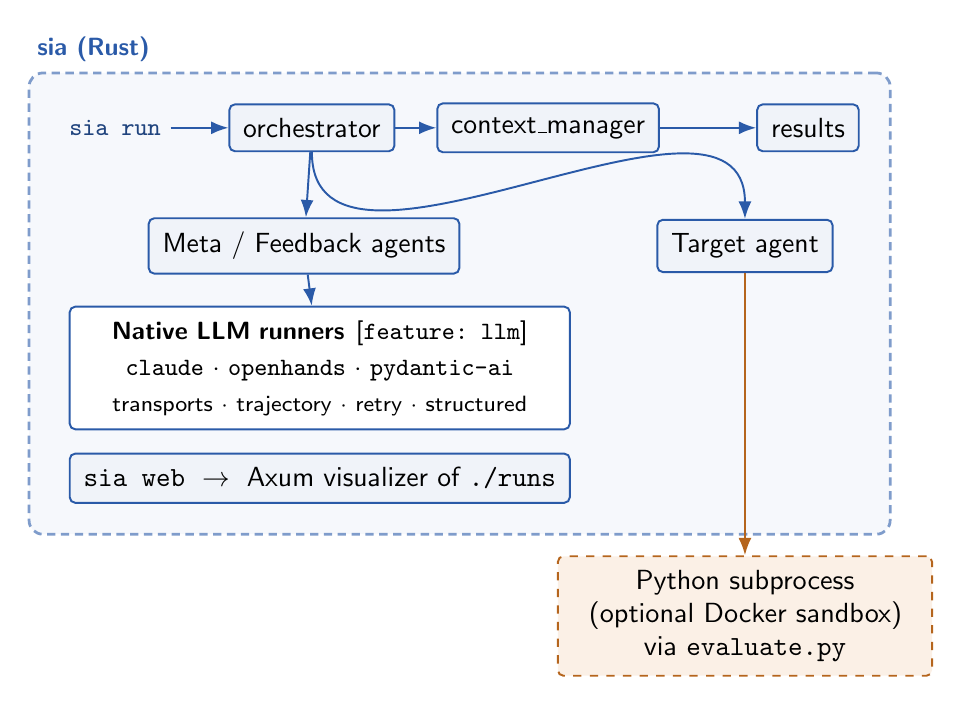
\begin{tikzpicture}[
  box/.style={rounded corners=2pt, draw=accent, fill=accent!7, line width=0.7pt,
              inner sep=5pt, align=center, font=\sffamily},
  lite/.style={rounded corners=2pt, draw=accent, fill=white, line width=0.7pt,
               inner sep=5pt, align=center, font=\sffamily\small},
  py/.style={rounded corners=2pt, draw=pyaccent, fill=pybg, line width=0.7pt, dashed,
             inner sep=5pt, align=center, font=\sffamily},
  entry/.style={font=\ttfamily\small, text=accent!75!black},
  flow/.style={-{Latex[length=2.2mm]}, draw=accent, line width=0.7pt},
  pyflow/.style={-{Latex[length=2.2mm]}, draw=pyaccent, line width=0.8pt},
]
% top pipeline
\node[entry] (run) at (0,4.3) {sia run};
\node[box] (orch) at (2.5,4.3) {orchestrator};
\node[box] (cm) at (5.5,4.3) {context\_manager};
\node[box] (res) at (8.8,4.3) {results};
% left branch: meta/feedback -> native runners
\node[box] (agents) at (2.4,2.8) {Meta / Feedback agents};
\node[lite, text width=6.0cm] (runners) at (2.6,1.25)
  {\textbf{Native LLM runners}\,\;[\texttt{feature: llm}]\\[2pt]
   \texttt{claude} $\cdot$ \texttt{openhands} $\cdot$ \texttt{pydantic-ai}\\[2pt]
   {\footnotesize transports $\cdot$ trajectory $\cdot$ retry $\cdot$ structured}};
% right branch: target agent (in Rust) -> Python subprocess (outside boundary)
\node[box] (target) at (8.0,2.8) {Target agent};
\node[box] (web) at (2.6,-0.15) {\texttt{sia web} $\;\to\;$ Axum visualizer of \texttt{./runs}};
% rust trust boundary (encloses all native components)
\begin{scope}[on background layer]
  \node[rounded corners=5pt, draw=accent!60, line width=1pt, dash pattern=on 3pt off 2pt,
        fill=accent!4, fit=(run)(res)(runners)(web)(target), inner sep=11pt] (rust) {};
\end{scope}
\node[anchor=south west, font=\sffamily\bfseries\small, text=accent] at (rust.north west)
  {sia (Rust)};
% Python subprocess: outside the boundary
\node[py, text width=4.4cm] (py) at (8.0,-1.9)
  {Python subprocess\\(optional Docker sandbox)\\via \texttt{evaluate.py}};
% arrows
\draw[flow] (run) -- (orch);
\draw[flow] (orch) -- (cm);
\draw[flow] (cm) -- (res);
\draw[flow] (orch) -- (agents);
\draw[flow] (agents) -- (runners);
\draw[flow] (orch.south) to[out=-90,in=90] (target.north);
\draw[pyflow] (target) -- (py);
\end{tikzpicture}%
}
\caption{The \texttt{sia\_rust} architecture. Native Rust meta/feedback runners drive
the LLM agents inside the trusted boundary; the Target-Agent is always executed as a
separate Python subprocess (optionally Docker-sandboxed) via the \texttt{evaluate.py}
contract.}
\label{fig:arch}
\end{figure}

This phased design --- native meta/feedback runners, a Python bridge only for target
execution --- yields safety and performance gains while preserving the task contract
existing custom tasks rely on.

\subsection{The native LLM layer}
The LLM layer (\texttt{src/llm/}, feature \texttt{llm}) centers on a small
synchronous \texttt{AgentRunner} trait (\texttt{src/llm/mod.rs}) returning a final
text plus a captured \texttt{AgentTrajectory}. Three native runners implement the
meta/feedback agents:

\begin{itemize}
\item \textbf{claude} (\texttt{src/llm/claude\_runner.rs}): a direct
  \texttt{/v1/messages} tool-use loop. A thin Messages-API client is used rather than
  \texttt{rig}'s agent abstraction so the loop has an injectable transport
  (\texttt{MessagesTransport}), exact \texttt{tool\_use} / \texttt{tool\_result}
  block plumbing, and \texttt{stop\_reason} control flow --- all testable offline
  with scripted responses.
\item \textbf{openhands} (\texttt{src/llm/openhands\_runner.rs}): an
  OpenAI-compatible chat-completions loop exposing \texttt{terminal} and
  \texttt{file\_editor} tools, persisting events in the OpenHands
  \texttt{openhands\_trajectory/.../events/event-*.json} shape that the web
  visualizer renders. It is the native replacement for the Python OpenHands (litellm)
  integration; model-spec routing to an OpenAI-compatible \texttt{base\_url} is
  handled by \texttt{HttpChatTransport} plus \texttt{resolve\_model} prefixing.
\item \textbf{pydantic-ai} (\texttt{src/llm/pydantic\_ai\_runner.rs}): a
  \texttt{write\_file} / \texttt{read\_file} / \texttt{bash} loop with a request limit
  matching Python's \texttt{UsageLimits(request\_limit=max\_turns)}. It reuses the
  in-tree OpenAI-compatible transport, shared tool executors, and trajectory
  middleware rather than taking a new agent dependency.
\end{itemize}

All three reuse the shared sandboxed \texttt{Bash} / \texttt{Read} / \texttt{Write} /
\texttt{Edit} / \texttt{Glob} executors in \texttt{src/llm/tools.rs}.

\subsection{Trajectory middleware}
\texttt{TrajectoryMiddleware} (\texttt{src/llm/trajectory\_middleware.rs}) is a
reusable observer that records structured \texttt{TrajectoryEvent}s (user prompt,
assistant text turns, tool calls, tool results, errors) and tracks token usage and
wall-clock timing. It mirrors each event into an \texttt{AgentTrajectory} via that
type's public \texttt{push\_*} builders, so it reuses the trajectory storage rather
than reinventing it, and its output is in the exact \texttt{agent\_execution.json}
shape the orchestrator reads back with no adapter. API-reported usage captured here
is the single source of truth for telemetry (Section~\ref{sec:telemetry}).

\subsection{Provider mapping}
\texttt{provider\_mapping.rs} is a single source of truth from a \texttt{Provider}
config to a constructed transport. It resolves the \texttt{client\_kind} (anthropic /
openai / google), the API-key env var, and a per-kind base-URL default (anthropic
$\rightarrow$ \texttt{api.anthropic.com}, openai $\rightarrow$
\texttt{api.openai.com/v1}, google $\rightarrow$ the OpenAI-compatible
\texttt{generativelanguage.googleapis.com/...} endpoint driven through the chat
transport), and emits helpful user-facing errors. This removes hand-rolled transport
construction from the individual runners.

\subsection{Retry / resilience}
\texttt{retry.rs} provides a deterministic exponential-backoff \texttt{RetryPolicy}
(jitter is applied only in the sleeping path so the schedule itself is exactly
unit-testable), a transient-error classifier, a reusable retry loop with an
\texttt{on\_attempt\_failed} hook for trajectory capture, and
\texttt{RetryMessagesTransport} / \texttt{RetryChatTransport} decorators that
implement the same transport traits as what they wrap (so retry is drop-in) and
support an optional secondary-transport fallback. Backoff is synchronous
(\texttt{std::thread::sleep}) to match the blocking transports' call sites.

\subsection{Structured-output parity}
\texttt{structured.rs} provides offline structured-output extraction plus a wrapper
over \texttt{rig-core}'s \texttt{Extractor} for the live path. It mirrors the Python
GPQA reference's \texttt{parse\_answer\_letter} semantics:
\texttt{.strip().upper()} normalization of the structured \texttt{answer} field, a
fall-back to raw-text uppercasing on JSON-parse failure, a final letter that is the
value if it is exactly one of A--D else the first A--D letter scanning
left-to-right, and a non-raising empty-string fallback when no A--D letter is
present.

\subsection{Telemetry}
\label{sec:telemetry}
\texttt{telemetry.rs} turns the run metrics the runners already capture (token usage,
tool calls, timing) into per-generation \texttt{GenerationTelemetry} plus a
cumulative summary, written as a \texttt{telemetry.json} artifact next to
\texttt{agent\_execution.json}. It performs no re-accounting --- the API-reported
usage recorded by the trajectory middleware is the single source of truth --- and
deliberately records \textbf{no} dollar-cost field because per-provider pricing is
unknown.

\subsection{SIA Studio}
The web layer (\texttt{src/web/server.rs}, \texttt{src/web/runs.rs}) is an Axum app
--- the ``SIA Studio'' dashboard --- that serves the runs visualizer over the
\texttt{runs/} directory, with routes for listing runs, run detail, evaluation
details, artifacts, and trajectories. It can run in the foreground (\texttt{sia web})
or on a daemon thread so the orchestrator can expose a live dashboard during
\texttt{sia run}. The bundled single-page UI is embedded at build time via
\texttt{include\_dir}.

\subsection{Capability sandbox + threat model}
\texttt{SECURITY.md} is a formal threat model for self-modifying agents: it
enumerates assets (host filesystem, environment secrets, network egress, host
compute, run integrity), three trust boundaries (trusted orchestrator; semi-trusted
LLM-driven native runner tools; untrusted Python target subprocess), escalation
paths (filesystem escape, network exfiltration, resource exhaustion,
prompt-injection-driven tool abuse), current mitigations, and a three-stage
OS-enforcement roadmap.

\texttt{src/sandbox.rs} implements stage 1: a pure-\texttt{std}, dependency-free
\texttt{Capabilities} allow-list compiled on the \textbf{default} build. It is
deny-by-default (read/write only within a declared \texttt{fs\_root}, \texttt{Bash}
gated, network denied, a per-file size cap) with \texttt{permissive} and
\texttt{read\_only} presets, and exposes \texttt{check\_read} / \texttt{check\_write}
/ \texttt{check\_bash} / \texttt{check\_within\_root} / \texttt{check\_size}. It is
the single auditable enforcement point the landlock/WASI roadmap builds on.
Crucially, it is \textbf{advisory and in-process}: it raises the bar against
injection and accidental escape but does not constrain a process that ignores it
(Section~\ref{sec:limitations}).

\subsection{Verifier layer}
\texttt{src/verifier.rs} defines a \texttt{Verifier} trait and reusable,
fully-offline verifiers that score a single \texttt{(submission, reference)} pair
without spawning Python, using the same $[0,1]$ semantics as the Python
\texttt{evaluate.py} \texttt{accuracy} field so the two are directly comparable. The
Python \texttt{evaluate.py} remains the authoritative system-of-record for
whole-dataset aggregation; the native path is scoped to unit-level checks. To make
the SIA paper's verifier-quality (Goodhart) concern testable, the module ships
\texttt{adversarial\_variants} (semantically-equivalent perturbations: whitespace,
case, trailing punctuation, wrapping prose) and \texttt{is\_stable} (asserts a
verifier returns the same outcome across all variants); every verifier is panic-free
on malformed input, returning a failing outcome rather than erroring.

\subsection{Heuristic adaptive scheduler}
\texttt{src/scheduler.rs} targets the SIA paper's harness-vs-weight decision-policy
future-work item with a deliberately simple, deterministic \textbf{heuristic}. For
each lever it defines an ``improvement efficiency'' metric --- mean positive score
improvement per unit of compute over consecutive same-lever generations --- and a
transparent decision tree (\texttt{decide\_next}) that reuses the weight module's
plateau detector and an efficiency comparison to recommend the next
\texttt{UpdateKind}. It is explicitly \textbf{not} meta-RL (no learned policy, no
environment, no gradient over the decision) and ships as a standalone, tested module
\textbf{not yet wired into the orchestrator}; the intended hookup (record
per-generation, decide before the next generation, surface an efficiency summary in
SIA Studio) is documented as a seam.

\subsection{Native weight-update abstraction + CPU reference}
\texttt{src/weights.rs} provides the honest first step toward weight updates: a
\texttt{WeightUpdater} abstraction, \texttt{TrainingExample} extraction from
high-reward trajectories, a \texttt{should\_trigger\_weight\_update} trigger seam,
and \texttt{LoraReferenceUpdater} --- a tested, pure-\texttt{f64}, fully-offline CPU
reference that runs LoRA gradient mechanics end-to-end
(\texttt{W\_eff = (B$\cdot$A)$\cdot$(alpha/rank)}, gradients through both factors,
decreasing loss on a learnable signal). It is explicitly a \textbf{reference}, not a
GPU trainer: it embeds examples into a small fixed-dimensional feature vector and
does reward-weighted MSE gradient descent; it does \textbf{not} load a real model,
run on a GPU, or update a real LLM's parameters. The intended real backend is Candle
behind a future non-default cargo feature; it is not depended on here because
\texttt{candle-core} is not in this build's offline cargo cache. The Python bridge is
\textbf{not} a training path --- this module spawns no subprocess and touches no
Python.

\section{Implementation \& Engineering}

\subsection{Feature-gated \texttt{llm} build}
The entire native LLM layer is gated behind the non-default \texttt{llm} cargo
feature (\texttt{Cargo.toml}:
\texttt{llm = ["dep:rig-core", "dep:reqwest", "dep:glob", "dep:schemars"]}) so the
default build and published crate stay dependency-light. Without the feature, the
meta/feedback runners return a clear ``build with \texttt{--features llm}'' message
and everything else (orchestration, web UI, parity) still works. CI exercises
\textbf{both} the default build and \texttt{--features llm}.

\subsection{Injectable-transport offline testability}
\label{sec:offline}
Every native tool-use loop is driven through an injectable transport
(\texttt{MessagesTransport} / \texttt{ChatTransport}). In-test mock transports return
scripted response sequences, so the full loops --- including tool execution,
tool-result feedback, and \texttt{stop\_reason} control flow --- are tested offline
with no network and no API keys. Real-provider calls are \texttt{\#[ignore]}d and
gated on the relevant API key. The end-to-end test
(\texttt{tests/end\_to\_end\_llm.rs}) proves the native loops integrate with the
artifacts the orchestrator/context pipeline consume and that dispatch routes to the
native runners rather than the feature-off boundary error.

\subsection{Byte-parity methodology}
\label{sec:parity-method}
\texttt{src/pyjson.rs} reproduces CPython's
\texttt{json.dumps(..., ensure\_ascii=True)} exactly, including the
\texttt{\textbackslash uXXXX} escaping needed for CJK content (e.g.\ LawBench). The
\texttt{sia-parity} binary (\texttt{src/bin/sia\_parity.rs}) emits the Rust output
for a given operation from a JSON request on stdin;
\texttt{scripts/parity\_check.py} runs the reference Python implementation and the
Rust helper on the same inputs --- \texttt{json.dumps} with indent, meta/feedback
prompts, feedback context, and execution-log loading --- over an ASCII + CJK + emoji
+ control-character matrix and asserts byte-identical output. This parity gate runs
in CI on every push.

\subsection{Embedding and dual-build CI}
Package-data that Python loaded via \texttt{importlib.resources} (bundled
provider/profile JSON and the web \texttt{index.html}) is embedded at build time via
\texttt{include\_dir}. CI (\texttt{.github/workflows/rust.yml}) runs
\texttt{cargo fmt --check}, \texttt{cargo clippy -D warnings}, and \texttt{cargo
test} for both the default and \texttt{--features llm} builds, plus the
differential-parity gate and the standalone \texttt{evals/} crate.

\section{Evaluation}
We report only what the repository actually measures. We do \textbf{not} report any
live self-improvement accuracy study (Section~\ref{sec:noteval}).

\subsection{Differential parity (fidelity)}
\texttt{scripts/parity\_check.py} asserts byte-identical output between the reference
Python implementation and the Rust port across the operations in
Section~\ref{sec:parity-method}, over an ASCII + CJK + emoji + control-character
matrix (e.g.\ the Chinese-charge LawBench-style fixture \texttt{故意伤害罪}, the
\texttt{ok $\checkmark$ [emoji] done} emoji fixture, and a
\texttt{\textbackslash t\textbackslash n\textbackslash r} control-char fixture). The
byte-for-byte criterion --- rather than semantic equality --- is what lets the same
web visualizer and context-loading code consume native and ported outputs
interchangeably. The port was developed red$\rightarrow$green with every Python test
and all seven golden-master files mirrored in Rust.

\subsection{Microbenchmarks (core-operation speed)}
Deterministic core operations are measured in both languages with byte-identical
fixtures (Rust via Criterion \texttt{cargo bench --bench core}; Python via
\texttt{benchmarks/bench\_python.py}); \texttt{benchmarks/run\_comparison.py}
regenerates \texttt{benchmarks/REPORT.md}. LLM calls are neutralized on both sides so
the benchmark isolates the deterministic core. On the machine recorded in
\texttt{benchmarks/REPORT.md} (4-core Xeon @ 2.80\,GHz, Linux, CPython 3.11.15,
rustc 1.94.1), the reported figures are given in Table~\ref{tab:bench}.

\begin{table}[t]
\centering
\caption{Core-operation microbenchmarks (ns/op) on the recorded machine. Speedups
are order-of-magnitude indicators, not portable constants (see text).}
\label{tab:bench}
\begin{tabular}{lrrr}
\toprule
\textbf{Operation} & \textbf{Python ns/op} & \textbf{Rust ns/op} & \textbf{Speedup} \\
\midrule
\texttt{build\_meta\_prompt}              & 13,616    & 551.4     & 24.7$\times$ \\
\texttt{build\_feedback\_prompt}          & 1,357     & 519.9     & 2.6$\times$ \\
\texttt{context\_manager\_run}            & 1,260,413 & 1,041,368 & 1.2$\times$ \\
\texttt{build\_feedback\_context\_single} & 200,225   & 14,333    & 14.0$\times$ \\
\texttt{build\_feedback\_context\_multi}  & 283,415   & 27,682    & 10.2$\times$ \\
\texttt{load\_agent\_execution\_single}   & 125,182   & 6,997     & 17.9$\times$ \\
\texttt{load\_agent\_execution\_multi}    & 199,860   & 25,149    & 7.9$\times$ \\
\texttt{web\_list\_runs}                  & 3,485,486 & 1,956,338 & 1.8$\times$ \\
\texttt{web\_get\_run}                    & 684,079   & 253,380   & 2.7$\times$ \\
\bottomrule
\end{tabular}
\end{table}

The \textbf{geometric-mean speedup across the nine operations is ${\sim}5.8\times$},
with prompt building up to ${\sim}25\times$ and execution-log loading up to
${\sim}18\times$. As \texttt{benchmarks/REPORT.md} itself cautions, the ns/op figures
mix CPU work with filesystem I/O for the fs-backed ops and are sensitive to machine
load and OS file-cache state, so these speedups should be read as order-of-magnitude
indicators on this machine, not precise or portable constants. They characterize the
deterministic scaffolding only and say nothing about end-to-end run time, which is
dominated by model inference latency.

\subsection{Test coverage}
The native loops are covered by offline mocked tool-loop tests
(Section~\ref{sec:offline}). The trajectory types support golden-master round-trips:
middleware output renders into the \texttt{agent\_execution.json} shape and is read
back by \texttt{load\_agent\_execution} without an adapter. Where the Python tests
patch \texttt{subprocess.run} / \texttt{subprocess.Popen}, the Rust port exposes
injectable seams (\texttt{run\_evaluation\_with}, \texttt{run\_target\_agent\_with},
\texttt{run\_generation\_with}) so the branching logic is unit-tested without a real
interpreter. The standalone \texttt{evals/} crate runs a GPQA-style \texttt{dspy-rs}
pipeline fully offline via a deterministic mock adapter, asserting a perfect mock
scores 100\% and an always-``A'' mock scores the expected lower value (20\% on the
bundled five-question fixture); it also offers a real-provider path. These are
infrastructure/correctness tests, \textbf{not} a self-improvement accuracy study.

\subsection{What is NOT evaluated}
\label{sec:noteval}
There is \textbf{no} live end-to-end self-improvement study here: we do not report
that the loop raises task accuracy across generations, nor any scheduler ablation,
nor any real weight-update training run. The scheduler and weight modules are tested
in isolation and are not yet wired into the orchestrator; the weight updater is a CPU
reference, not a real-model trainer. A runnable example task exists, but it is a
demonstration, not a benchmark study. Producing such studies is future work
(Section~\ref{sec:future}).

\subsection{Reproducibility statement}
The repository defines a single authoritative reproducibility standard in
\texttt{docs/REPRODUCIBILITY.md}: the exact per-run and per-generation artifact set
(real filenames + JSON schemas), the mandatory metadata to report (git commit,
profiles, model slugs, provider/\texttt{client\_kind}, task, generation count), and a
third-party verification path that separates \emph{verifying the implementation}
(offline, no keys: \texttt{cargo test}, the \texttt{scripts/parity\_check.py} parity
gate, and \texttt{sia web}) from \emph{reproducing a live run} (keys required). It is
explicit that, because LLM sampling is involved and \textbf{no random seed is set or
recorded}, live runs are not bit-reproducible: reproducibility here means the same
artifact set/schema plus the byte-parity-tested deterministic core
(Section~\ref{sec:noteval} notwithstanding), not identical model text. Consistent
with the above, a live end-to-end run remains \textbf{unvalidated} (issue~\#93).

\section{Discussion, Limitations \& Future Work}

\subsection{Limitations (today)}
\label{sec:limitations}
\begin{itemize}
\item \textbf{Bash / sandbox gaps.} The native \texttt{Bash} tool runs arbitrary
  \texttt{sh -c} commands with only a wall-clock timeout --- no command allow-list,
  no network restriction, no memory/CPU cap at that layer --- and is \textbf{not yet
  wired} to the capability layer's \texttt{check\_bash}. The lexical path sandbox
  blocks \texttt{..} and absolute paths but \textbf{does not resolve symlinks}
  (TOCTOU/symlink traversal remain possible). The capability layer
  (\texttt{src/sandbox.rs}) is \textbf{advisory and in-process}, not kernel-enforced.
  The default \texttt{--sandbox none} offers no confinement for the target
  subprocess; \texttt{--sandbox docker} (network-none, read-only dataset, cpu/mem
  caps) is the recommended mode for untrusted tasks. The Claude SDK runner path uses
  \texttt{bypassPermissions} to enable automation.
\item \textbf{Heuristic scheduler.} The harness-vs-weight scheduler is a
  deterministic heuristic, not a learned policy, and is not yet wired into the
  orchestrator. UCB / contextual-bandit / meta-RL stages are \textbf{not
  implemented}.
\item \textbf{Reference-only weight updates.} \texttt{src/weights.rs} is an
  abstraction plus a CPU \texttt{f64} reference LoRA that does not touch a real model
  or GPU. Candle is not integrated (it is not in the offline cargo cache).
\item \textbf{No live improvement benchmark.} As stated in
  Section~\ref{sec:noteval}.
\item \textbf{Benchmark portability.} The speedups are single-machine and mix CPU
  with I/O.
\end{itemize}

\subsection{Future work}
\label{sec:future}
\begin{itemize}
\item \textbf{Full meta-RL scheduler.} Replace the heuristic \texttt{decide\_next}
  (keeping its shape) with a learned harness-vs-weight policy; the intermediate UCB
  and contextual-bandit stages named in the project roadmap are the natural staging
  path and remain unimplemented.
\item \textbf{Candle GPU LoRA.} A \texttt{CandleLoraUpdater} implementing
  \texttt{WeightUpdater} behind a non-default \texttt{weights-gpu}/\texttt{candle}
  feature \citep{candle}, reusing the existing trait, \texttt{TrainingExample}
  extraction, and trigger unchanged, to perform real weight-update training from
  high-reward trajectories.
\item \textbf{OS-level sandboxing.} Stage 2 (a Linux \texttt{landlock} filesystem
  ruleset scoped to \texttt{fs\_root} plus a \texttt{seccomp} syscall filter, behind
  a \texttt{landlock-sandbox} feature) and stage 3 (running untrusted generated
  agents as WASI preview2 components under \texttt{wasmtime} \citep{wasmtime} with
  only preopened directories and no ambient authority) --- each \emph{enforcing} the
  capability policy at a lower level so a tool-layer bug cannot ignore it. A code
  sketch exists in \texttt{src/sandbox.rs}; neither stage is wired in (the
  \texttt{landlock} crate is not in the offline cache).
\item \textbf{End-to-end studies.} Once the scheduler and a real weight backend are
  wired into the orchestrator, run live multi-generation self-improvement studies
  (accuracy-vs-generation curves, scheduler ablations, cost/telemetry analysis) on
  the bundled tasks. None of this is claimed here.
\end{itemize}

\section{Related Work}
The closest prior work is the original \textbf{SIA} framework
\citep{hebbar2026sia}, which defines the meta/target/feedback loop, the
harness-vs-weight-update distinction, and the future-work and verifier-quality
concerns this work engages with; \texttt{sia\_rust} is a native Rust
re-implementation plus the extensions above. The native agent layer is built on
\textbf{rig-core} \citep{rigcore}, and the eval crate on \textbf{dspy-rs / DSRs}
\citep{dsrs}, the Rust port of DSPy. The roadmap toward stronger isolation references
\textbf{Candle} \citep{candle} for native-Rust ML, and \textbf{landlock},
\textbf{seccomp}, and \textbf{WASI/wasmtime} \citep{wasmtime} for OS- and VM-level
enforcement. We keep this section modest and cite tools by their repositories rather
than attributing them to papers we have not verified.

\section{Conclusion}
\texttt{sia\_rust} is a native Rust re-implementation of the SIA
self-improving-agent framework whose deterministic core reproduces the reference
Python implementation's prompt, context, and execution-log output
\textbf{byte-for-byte}, layered with a native multi-provider LLM agent-runner stack
(three runners, injectable transports, trajectory middleware, provider mapping,
retry, structured-output parity) and a set of honestly-scoped safety, observability,
and scheduling extensions (capability sandbox + threat model, native verifier,
telemetry, SIA Studio, a heuristic scheduler, and a CPU reference weight updater).
Our evaluation is fidelity (byte-parity), core-operation microbenchmarks
(${\sim}5.8\times$ geomean on the recorded machine), and offline test coverage ---
and we are explicit that full meta-RL scheduling, GPU LoRA training, OS-level sandbox
enforcement, and live end-to-end self-improvement studies are future work, not
present results. We offer this as an experience report on building a faster, safer,
more observable substrate for self-modifying agents, and as a stable set of seams
others can build those future results on.

\paragraph{Note on citations.} The SIA arXiv identifier is taken from this
repository's README badge and links. Tool references point to project repositories
rather than to papers, to avoid fabricating bibliographic details. The
\citet{hebbar2026sia} author list is intentionally minimal (\texttt{and others}) and
should be completed against the arXiv record before any external submission.

\bibliographystyle{unsrtnat}
\bibliography{references}

\end{CJK}
\end{document}
